\documentclass[a4paper,12pt,uplatex,dvipdfmx]{jsarticle}

% 数式
\usepackage{amsmath,amsfonts}
\usepackage{bm}
% グラフィック
\usepackage{graphicx}
\usepackage{tikz}

\usepackage{url}
\usetikzlibrary{intersections, calc, arrows}

\begin{document}

\title{ガンマ関数とベータ関数について}
\author{@Tdrj2716}
\date{\today}
\maketitle

自分の\LaTeX の練習も兼ね, 有名な関数であるガンマ関数とベータ関数についてまとめました. それぞれ階乗とコンビネーションを正の実数で一般化したものに相当します(実際にはガンマ関数は実部が正の複素数で定義されます)が, その事実がどのようにして導出できるのかをここでは扱います.

\section{ガンマ関数}
\subsection{定義}
正の実数$x$について, 次の積分で定義される関数
\[
  \Gamma(x) = \int_0^\infty t^{x-1}\mathrm{e}^{-t} dt
\]
をガンマ関数と呼ぶ. グラフは図\ref{fig:gamma}のようになる.
\begin{figure}
    \begin{center}
        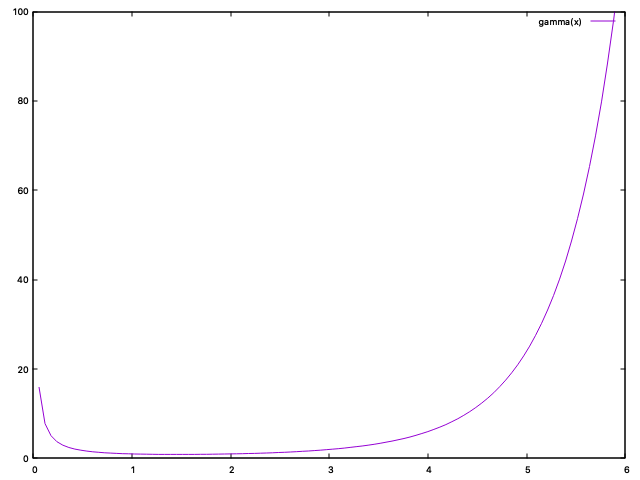
\includegraphics[clip, width=5cm]{gamma.png}
        \caption{ガンマ関数}
        \label{fig:gamma}
    \end{center}
\end{figure}

\subsection{性質:階乗の一般化}
任意の正整数$n$に対し, 次の式が成り立つ.
\[
    \Gamma(n+1) = n!
\]
(証明)
\[
    \Gamma(1) = \int_0^\infty \mathrm{e}^{-t} dt = \lim_{x \to \infty} [-\mathrm{e}^{-t}]_0^x = 1 = 0!
\]
また, 任意の正整数$n$に対して 
\begin{eqnarray*}
    \Gamma(n) & = & \int_0^\infty t^{n-1}\mathrm{e}^{-t} dt = [-t^{n-1}\mathrm{e}^{-t}]_0^{\infty} + \int_0^\infty (n-1)t^{n-2}\mathrm{e}^{-t} dt \\
    & = & \lim_{x \to \infty}[-t^{n-1}\mathrm{e}^{-t}]_0^x + (n-1)\int_0^\infty t^{n-2}\mathrm{e}^{-t} dt \\
    & = & 0 + (n-1)\Gamma(n-1) 
\end{eqnarray*}
よって, ~$\Gamma(n+1) = n\Gamma(n) = n!\Gamma(1) = n!$

\section{ベータ関数}
\subsection{定義}
\subsection{$x, y$ が自然数であるとき}
\subsection{ガンマ関数との関係}

\begin{thebibliography}{9}
    \bibitem{mathtrain-ガンマ}
    高校数学の美しい物語, ガンマ関数(階乗の一般化)の定義と性質 \\
    \url{https://mathtrain.jp/gamma}
    \bibitem{mathtrain-beta}
    高校数学の美しい物語, ベータ関数の積分公式 \\
    \url{https://mathtrain.jp/beta}
    \bibitem{ガンマ-beta}
    倭算数理研究所, ガンマ関数とベータ関数のよくある関係 \\
    \url{https://wasan.hatenablog.com/entry/20110623/1308805478#%E3%82%AC%E3%83%B3%E3%83%9E%E9%96%A2%E6%95%B0%E3%81%A8%E3%83%99%E3%83%BC%E3%82%BF%E9%96%A2%E6%95%B0%E3%81%AE%E9%96%A2%E4%BF%82%E5%BC%8F}
\end{thebibliography}

\end{document}